\chapter{Homology}
Before go into what \textit{persistent} homology it is well worth our time to clearly state what we mean by homology. (Why? Can this be skipped by experienced readers or are our definitions non-standard? Do we mostly follow hatcher?). In a general sense, homology is a particular of invariant of topological spaces. This has categorical reasons and others.
Importantly we need to define simplicial complexes. There are other ways of defining this, notably singular homology, but for the computational aspect of persistent homology we do not have to dwell on this. For completion, we refer the reader to Hatcher for a more traditional treatment of homology.

\section{Simplices}
First we start with the simplex.

\begin{figure}
  \centering
  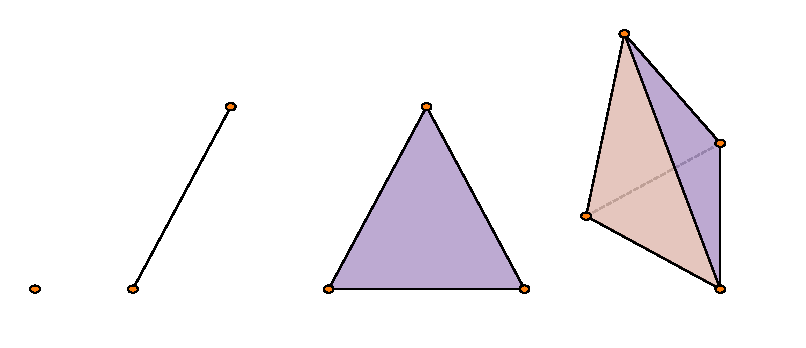
\includegraphics[]{simplex.pdf}
  \label{simplices}
  \caption{0-simplex (left), 1-simplex (middle left), 2-simplex (middle right) and 3-simplex (right).}
  \end{figure}
\begin{definition}
An $n$-simplex is the smallest possible convex set in $\mathbb{R}^{m}$ containing $n+1$ points $v_{0},\dots,v_{n}$ such that the vectors $v_{1}-v_{0}, \dots, v_{n} - v_{0}$ are linearily independent. The points $v_{0},\dots,v_{n}$ are known as the \textit{vertices} of the simplex.
\end{definition}
\begin{definition}
The \textit{standard} $n$-simplex is the $n$-simplex with vertices being the unit vectors along coordinate axes
\[ \Delta^{n} := \{ (t_{0}, \dots, t_{n}) \in R^{n+1} \mid \sum_{i} t_{i} = 1, t_{i} \geq 0 \quad \forall i \}
\]
\end{definition}

\begin{definition}
A face of a simplex is the convex hull of a subset of its vertices.
\end{definition}
\section{Simplicial complex}

\begin{definition}
A simplicial complex $K$ is a finite collection of simplices such that

\begin{enumerate}
    \item $\sigma \in K$ and $\tau \subset \sigma$ implies that $\tau \in K$
    \item $\sigma_{1}, \sigma_{2} \in K$ implies that $\sigma_{1} \cap \sigma_{2}$ is either empty or a face of both.
\end{enumerate}

\end{definition}
This is the geometric definition of a simplicial complex. However, since we are working with topological spaces it is advantageous to think of an abstract simplicial complex without concerning ourselves with the geometric connotations:

\begin{figure}
  \centering
  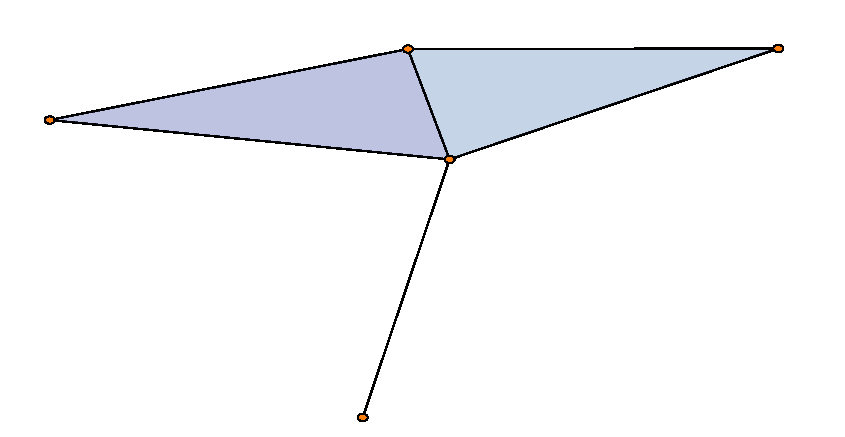
\includegraphics[scale=0.7]{complex.pdf}
  \label{complex}
  \caption{Example of a simplicial complex consisting of two 2-simplices glued together with an attached 1-simplex.}
\end{figure}

\begin{definition}[book]
An abstract simplicial complex $A$ is a finite collection of sets such that $\alpha \in A$ and $\beta \subseteq \alpha$ implies that $\beta \in A$.
\end{definition}

This abstract definition coincides with the geometric definition by calling the elements of $A$ its simplices. The simplices of $A$ are no longer geometric objects in Euclidean space, but simply combinatorial objects consisting of vertex sets.

It is easy to see how one can go from a geometric simplicial complex to an abstract simplicial complex simply by forgetting everything but the vertices themselves. However, most of the time our interest lies in the opposite direction: how do we go from an abstract simplicial complex to a geometric one? This is done by the geoemtric realization of $A$.

\begin{theorem}
Every abstract simplicial complex of dimension $d$ has a geometric realization in $\mathbb{R}^{2d+1}$.
\end{theorem}
\begin{proof}
See ?.
\end{proof}%
From here on we will simply refer to abstract simplicial complexes as a simplicial complex unless stated otherwise.
\section{Simplicial homology}
For a simplicial complex $K$ of dimension $n$ we define a free abelian group $C_{k}$ on the oriented $k-$simplices of $K$.
The elements of $C_{k}$ are called $k$-chains and are formal sums of the type
$\sum \alpha_{i} \sigma_{i}$
where $\alpha_{i}$ are coefficients in some ring $R$ and $\sigma_{i}$ are $k$-dimensional simplices. Furthermore, we have a collection of homomorphisms, known as boundary maps, which together with the groups form a chain complex. The $k$th boundary map
\[ \partial_{k}: C_{k} \to C_{k-1}\]
takes a $k$-simplex to its boundary
\[ \partial_{k} \sigma = \sum^{k}_{{i=0}} (-1)^{i} [v_{0},\dots,\hat v_{i}, \dots, v_{k}]\]
where $\hat v_{i}$ signifies that this vertex has been omitted. This is a homomorphism so
\[\partial_{k} \sum \alpha_{i}\sigma_{i} = \sum \alpha_{i} \partial_{k} \sigma_{i}\]

Now a simplicial chain complex is a collection of chain groups together with their corresponding boundary maps as a sequence:
\begin{center}
\begin{tikzcd}
  \dots \arrow[]{r}{\partial_{k+1}} & C_k \arrow[]{r}{\partial_{k}} & C_{k-1} \arrow[]{r}{\partial_{k-1}} & C_{k-2} \arrow[]{r}{\partial_{k-2}} & \dots
\end{tikzcd}
\end{center}
Note that the boundary maps compose to become the zero map.
\begin{theorem}
The composed boundary map $\partial_{k+1} \circ \partial_{k}$ is the zero map.
\end{theorem}
\begin{proof}
(Proof is in Hatcher)
\end{proof}
From this definition we know that from every simplicial complex $K$ we can associate a simplicial chain complex (this is a functor). We then define the $k$th homology group of $K$ as the quotient group
\[H_{k}(K) = Ker(\partial_{k})/Im(\partial_{k+1})\]

This is also a functor, so any simplicial map $K_{1} \to K_{2}$ induces a map on homology $H_{*}(K_{1}) \to H_{*}(K_{2})$.

TODO: Something about the coefficients. Expand on the sections above with examples of what cycles are etc.

%%% Local Variables:
%%% mode: latex
%%% TeX-master: "thesis.tex"
%%% End:
